\titlespacing{\section}{0pt}{12pt plus 4pt minus 2pt}{-6pt plus 2pt minus 2pt}

% Kopf- und Fusszeile
\renewcommand{\sectionmark}[1]{\markright{#1}}
\renewcommand{\leftmark}{\rightmark}
\pagestyle{fancy}
\lhead{}
\chead{}
\rhead{\thesection\space\contentsname}
\lfoot{Generative Testerstellung für Microservice-Architekturen}
\cfoot{}
\rfoot{Seite \thepage}
\renewcommand{\headrulewidth}{0.4pt}
\renewcommand{\footrulewidth}{0.4pt}

% Vorspann
\renewcommand{\thesection}{\Roman{section}}
\renewcommand{\theHsection}{\Roman{section}}
\pagenumbering{Roman}

% ----------------------------------------------------------------------------------------------------------
% Titelseite
% ----------------------------------------------------------------------------------------------------------
\thispagestyle{empty}
\begin{center}
	
\includegraphics[scale=0.25]{images/Hochschule_Muenchen_Logo.png}\\
	\vspace*{2cm}
	\Large
	\textbf{Fakultät für Informatik und Mathematik 07}\\
	\vspace*{2cm}
	\Huge
	\textbf{Bachelorarbeit}\\
	\vspace*{0.5cm}
	\large
	über das Thema\\
	\vspace*{1cm}
	\textbf{Generative Testerstellung für Microservice-Architekturen}\\
	\vspace*{2cm}
	
	\vfill
	\normalsize
	\newcolumntype{x}[1]{>{\raggedleft\arraybackslash\hspace{0pt}}p{#1}}
	\begin{tabular}{x{6cm}p{7.5cm}}
		\rule{0mm}{5ex}\textbf{Autor:} & Fabian Holtkötter\newline holtkoet@hm.edu \\ 
		\rule{0mm}{5ex}\textbf{Prüfer:} & Prof. Dr. Ulrike Hammerschall \\ 
		\rule{0mm}{5ex}\textbf{Abgabedatum:} & 03.03.2017 \\ 
	\end{tabular} 
\end{center}
\pagebreak

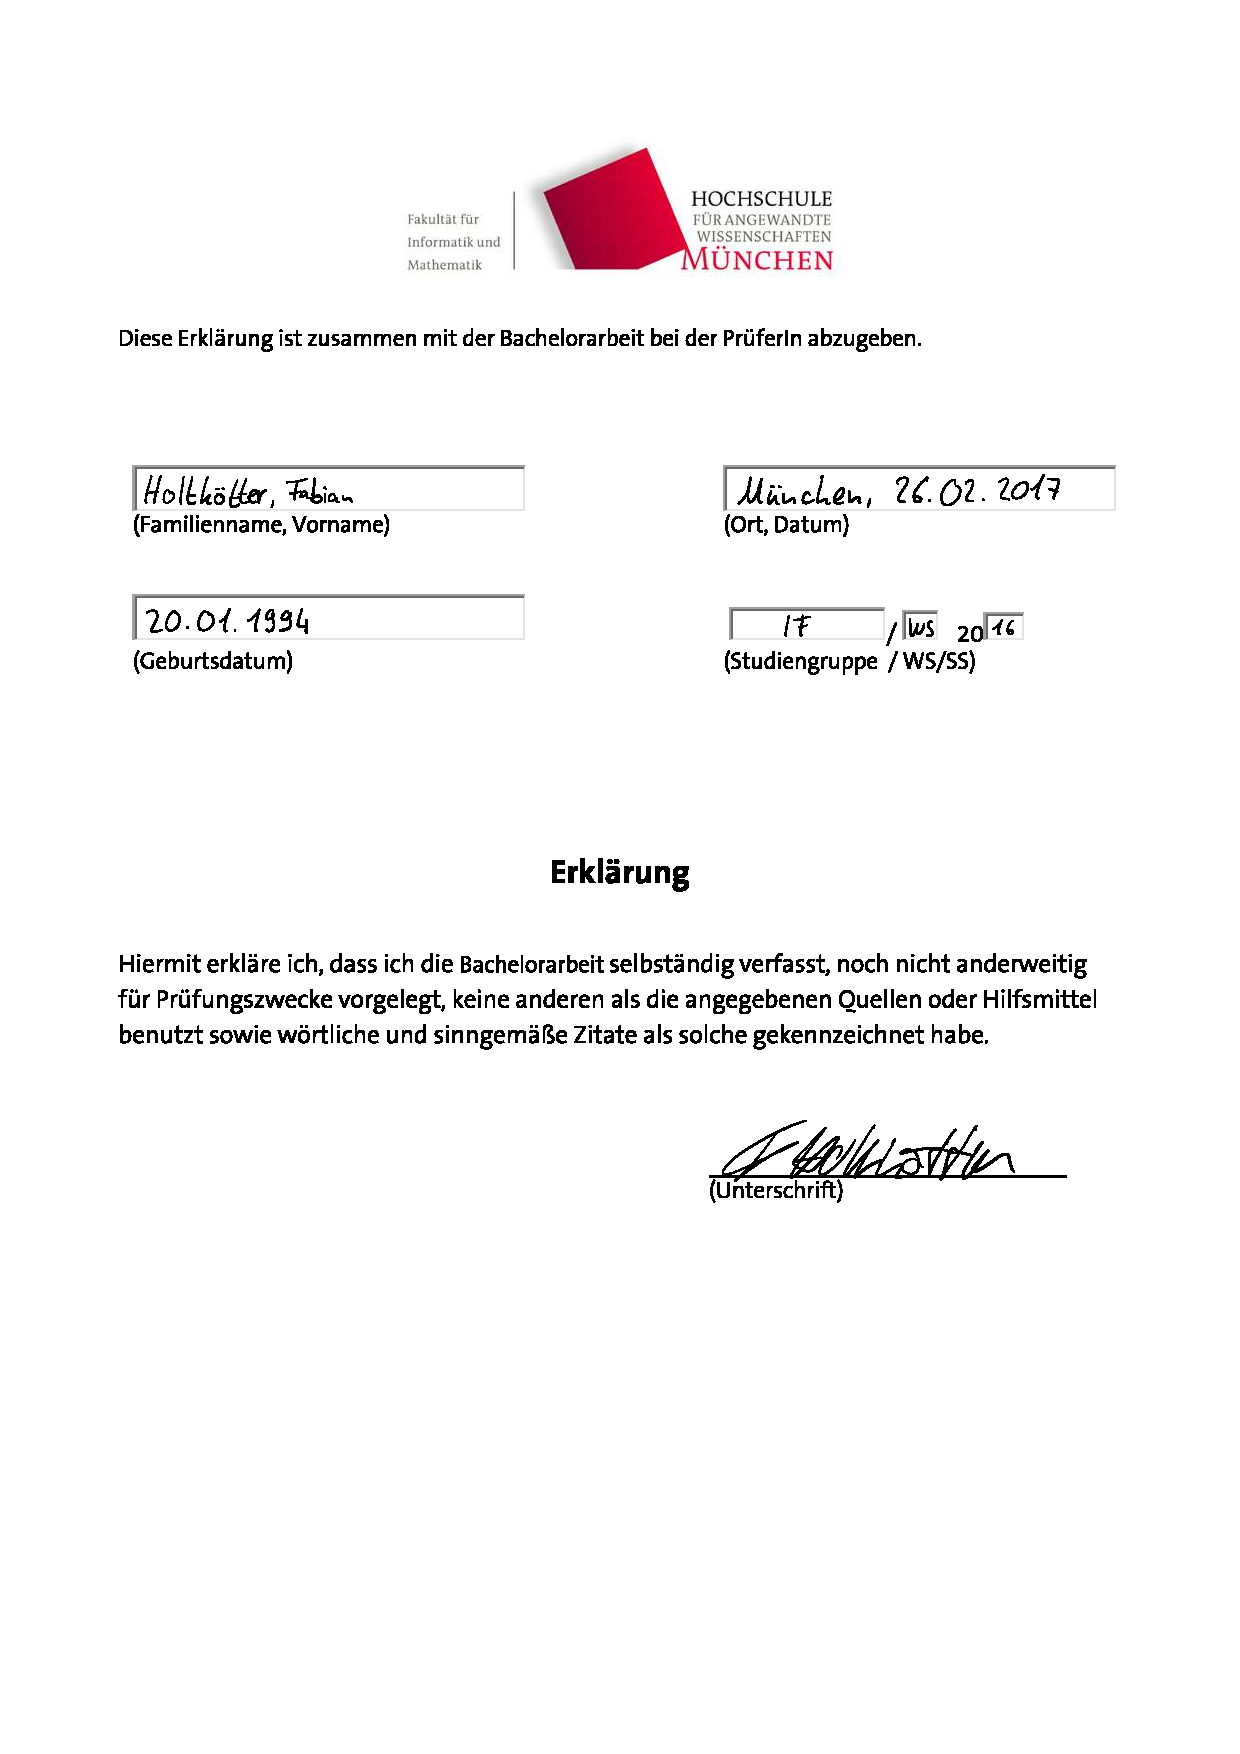
\includepdf{erklaerung.pdf}